% Integration snippets for director-helper-3; assets are under publication/methods-figures.
\begin{figure*}[tb]
\centering
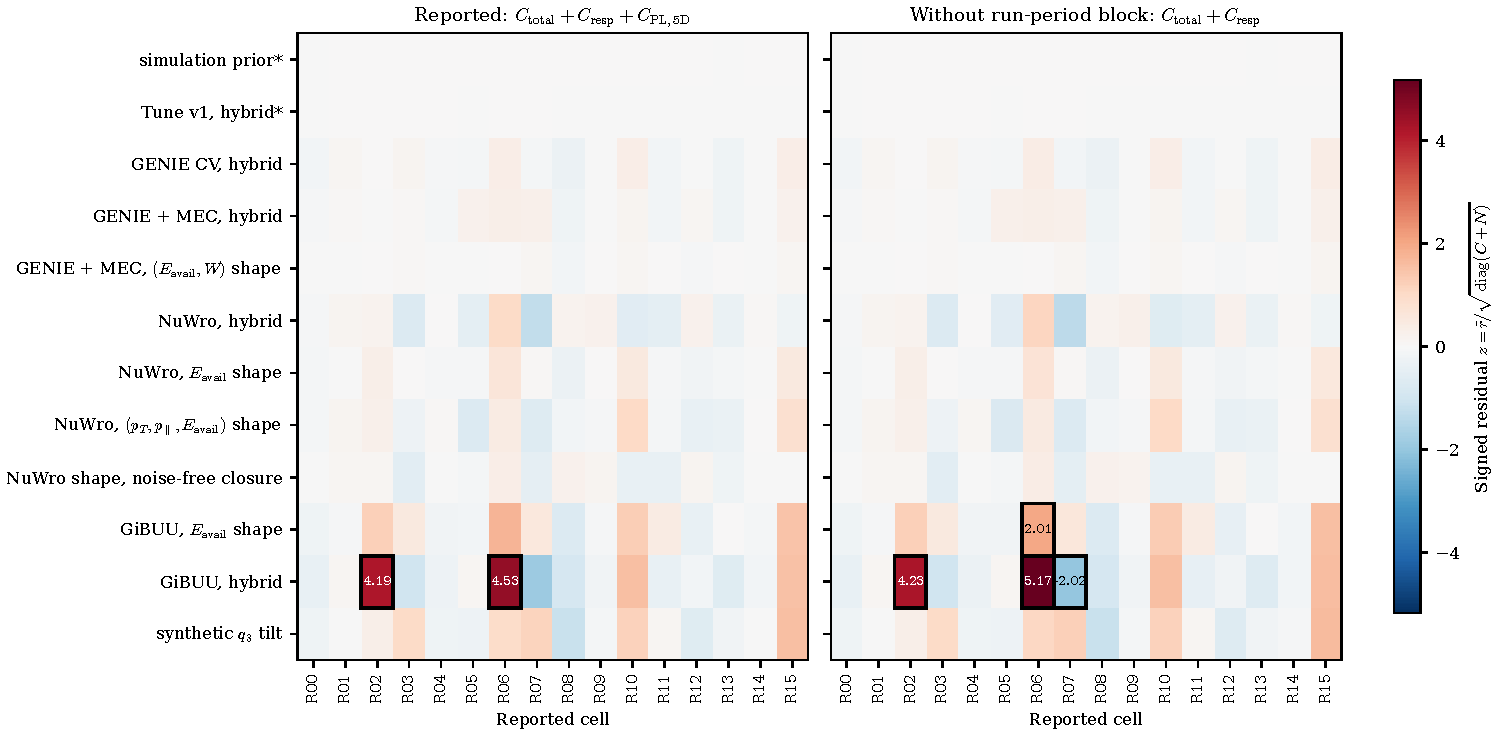
\includegraphics[width=\textwidth]{../../publication/methods-figures/paper_bias_cells.pdf}
\caption{Fake-data bias of the reported five-observable estimator on the sixteen cells, at the twelve graded truths of table~\ref{tab:fd16}, in the same order. Colour gives the signed residual $z=b/\sqrt{\mathrm{diag}(C+N)}$, where $b$ is the mean fractional residual and $N$ its noise covariance (the noise-free closure uses its single residual). Left uses the reported covariance, $C_{\mathrm{total}}+C_{\mathrm{resp}}+C_{\mathrm{PL,5D}}$; right omits the run-period block. Each covariance omits the truth's own generator component as in the table. Black outlines mark $|z|>2$. The bias is identical in both panels; only the covariance differs. An asterisk marks the simulation's own truth. These tests assess bias, not interval coverage; the joint $p$ criterion is reported in the table.}
\label{fig:bias-cells}
\end{figure*}
% Proposed citation: section 5.3, immediately before Table 2, retaining the complete table.

\begin{figure*}[tb]
\centering
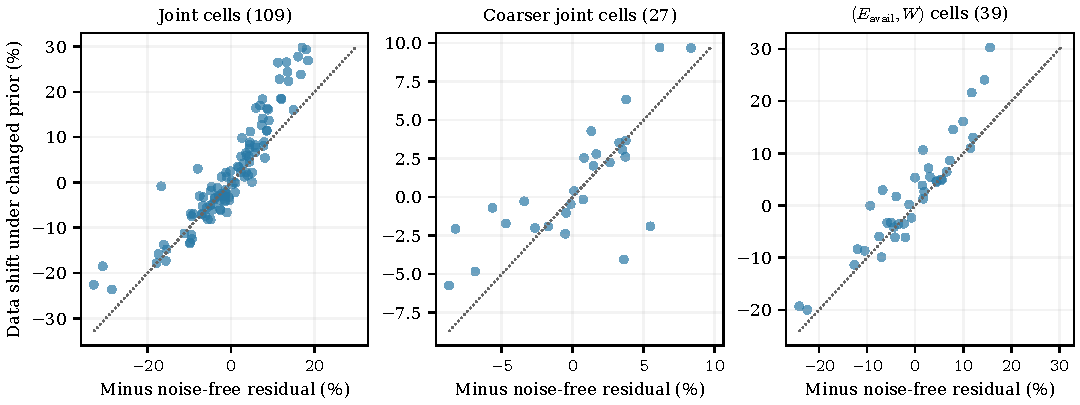
\includegraphics[width=\textwidth]{../../publication/methods-figures/paper_prior_response.pdf}
\caption{Sensitivity to the prior of the reported five-observable estimator at five iterations. The vertical axis is the relative change in the data result when the simulation prior is reweighted to the historical NuWro $(p_T,p_\parallel,E_{\mathrm{avail}})$ shape, divided by the result with the nominal prior. The horizontal axis is minus the noise-free fractional residual at that changed truth in signal-only simulation. Points are supported cells: 109 fine joint cells, 27 coarser joint cells and 39 $(E_{\mathrm{avail}},W)$ cells; they are not independent repeated experiments. The dotted line marks equality. The shifts measure sensitivity to the prior, not a measured bias of the data result, and their correlation with the simulated residual supplies no per-cell bias bound.}
\label{fig:prior-response}
\end{figure*}
% Proposed citation: section 7, after the sentence saying these shifts measure sensitivity to the prior.
